
\subsection{}
The system will become unstable when a delay of 0.4 seconds is used. The settling time for 0.39 is quite long but the system does stabilize. Figure \ref{fig:network_delay} shows different time delay settings in Simulink. It clearly shows that a delay of 0.3 seconds still makes the system stabilize quickly while a delay of 0.4 makes it unstable.

\begin{center}
      \begin{figure}[H]
      \centering
        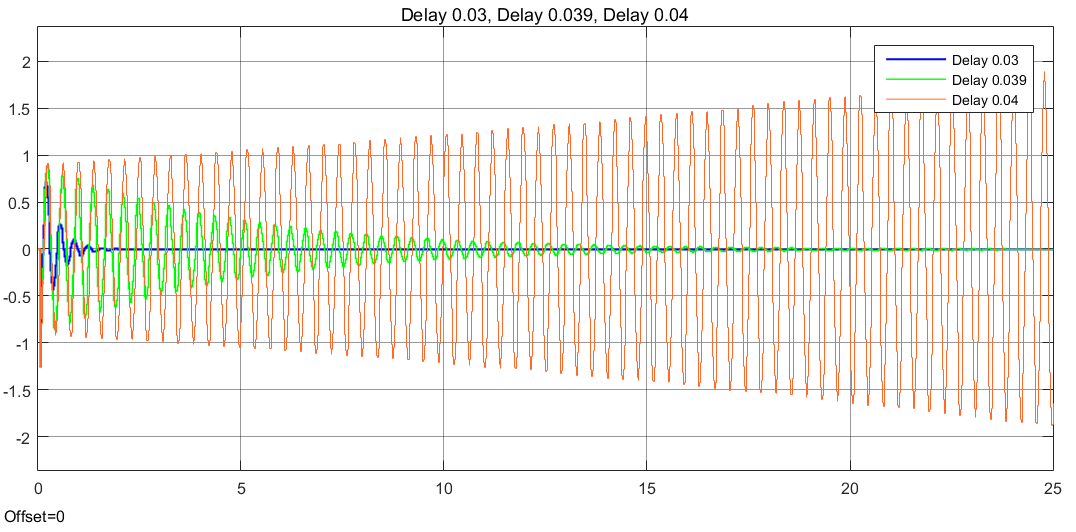
\includegraphics[scale=0.5]{network_delay.png}
        
      \caption{Control signal for different delay settings}
      \label{fig:network_delay}
      
      \end{figure}
    \end{center}
    
